\documentclass[10pt,]{article}
\usepackage[T1]{fontenc}
\usepackage{lmodern}
\usepackage{amssymb,amsmath}
\usepackage{ifxetex,ifluatex}
\usepackage{fixltx2e} % provides \textsubscript
% Set line spacing
% use upquote if available, for straight quotes in verbatim environments
\IfFileExists{upquote.sty}{\usepackage{upquote}}{}
\ifnum 0\ifxetex 1\fi\ifluatex 1\fi=0 % if pdftex
  \usepackage[utf8]{inputenc}
\else % if luatex or xelatex
  \ifxetex
    \usepackage{mathspec}
    \usepackage{xltxtra,xunicode}
  \else
    \usepackage{fontspec}
  \fi
  \defaultfontfeatures{Mapping=tex-text,Scale=MatchLowercase}
  \newcommand{\euro}{€}
\fi
% use microtype if available
\IfFileExists{microtype.sty}{\usepackage{microtype}}{}
\usepackage[margin=1in]{geometry}
\usepackage{color}
\usepackage{fancyvrb}
\newcommand{\VerbBar}{|}
\newcommand{\VERB}{\Verb[commandchars=\\\{\}]}
\DefineVerbatimEnvironment{Highlighting}{Verbatim}{commandchars=\\\{\}}
% Add ',fontsize=\small' for more characters per line
\usepackage{framed}
\definecolor{shadecolor}{RGB}{248,248,248}
\newenvironment{Shaded}{\begin{snugshade}}{\end{snugshade}}
\newcommand{\KeywordTok}[1]{\textcolor[rgb]{0.13,0.29,0.53}{\textbf{{#1}}}}
\newcommand{\DataTypeTok}[1]{\textcolor[rgb]{0.13,0.29,0.53}{{#1}}}
\newcommand{\DecValTok}[1]{\textcolor[rgb]{0.00,0.00,0.81}{{#1}}}
\newcommand{\BaseNTok}[1]{\textcolor[rgb]{0.00,0.00,0.81}{{#1}}}
\newcommand{\FloatTok}[1]{\textcolor[rgb]{0.00,0.00,0.81}{{#1}}}
\newcommand{\CharTok}[1]{\textcolor[rgb]{0.31,0.60,0.02}{{#1}}}
\newcommand{\StringTok}[1]{\textcolor[rgb]{0.31,0.60,0.02}{{#1}}}
\newcommand{\CommentTok}[1]{\textcolor[rgb]{0.56,0.35,0.01}{\textit{{#1}}}}
\newcommand{\OtherTok}[1]{\textcolor[rgb]{0.56,0.35,0.01}{{#1}}}
\newcommand{\AlertTok}[1]{\textcolor[rgb]{0.94,0.16,0.16}{{#1}}}
\newcommand{\FunctionTok}[1]{\textcolor[rgb]{0.00,0.00,0.00}{{#1}}}
\newcommand{\RegionMarkerTok}[1]{{#1}}
\newcommand{\ErrorTok}[1]{\textbf{{#1}}}
\newcommand{\NormalTok}[1]{{#1}}
\usepackage{graphicx}
% Redefine \includegraphics so that, unless explicit options are
% given, the image width will not exceed the width of the page.
% Images get their normal width if they fit onto the page, but
% are scaled down if they would overflow the margins.
\makeatletter
\def\ScaleIfNeeded{%
  \ifdim\Gin@nat@width>\linewidth
    \linewidth
  \else
    \Gin@nat@width
  \fi
}
\makeatother
\let\Oldincludegraphics\includegraphics
{%
 \catcode`\@=11\relax%
 \gdef\includegraphics{\@ifnextchar[{\Oldincludegraphics}{\Oldincludegraphics[width=\ScaleIfNeeded]}}%
}%
\ifxetex
  \usepackage[setpagesize=false, % page size defined by xetex
              unicode=false, % unicode breaks when used with xetex
              xetex]{hyperref}
\else
  \usepackage[unicode=true]{hyperref}
\fi
\hypersetup{breaklinks=true,
            bookmarks=true,
            pdfauthor={Filip Wójcik},
            pdftitle={Motor Trend analysis - is manual transmission or automatic transmission better for mpg?},
            colorlinks=true,
            citecolor=blue,
            urlcolor=blue,
            linkcolor=magenta,
            pdfborder={0 0 0}}
\urlstyle{same}  % don't use monospace font for urls
\setlength{\parindent}{0pt}
\setlength{\parskip}{6pt plus 2pt minus 1pt}
\setlength{\emergencystretch}{3em}  % prevent overfull lines
\setcounter{secnumdepth}{0}

%%% Change title format to be more compact
\usepackage{titling}
\setlength{\droptitle}{-2em}
  \title{Motor Trend analysis - is manual transmission or automatic transmission
better for mpg?}
  \pretitle{\vspace{\droptitle}\centering\huge}
  \posttitle{\par}
  \author{Filip Wójcik}
  \preauthor{\centering\large\emph}
  \postauthor{\par}
  \predate{\centering\large\emph}
  \postdate{\par}
  \date{Monday, May 18, 2015}




\begin{document}

\maketitle


\section{Summary}\label{summary}

After performing analysis, the cocnclusion is, that manual transmission
results in a bigger mpg value and consequently is a better option.
Change from automatic to manual transmission results in a approximately
2.9358 miles/gallon increase (when taken into account along with vehicle
weight and calculate on the 1/4 mile time).

\section{Exploratory data analysis}\label{exploratory-data-analysis}

Exploratory data analysis plots (for each variable) can be found as
\textbf{Figure1} in an appendix.

\section{Is an automatic or manual transmission better for
MPG}\label{is-an-automatic-or-manual-transmission-better-for-mpg}

\textbf{Figure2 (boxplot of mpg means between two groups)} and
\textbf{figure3 (correlation plot)} from appendix shows the difference
in mpg values between two groups - with manual and automatic
transmission. From the plot we can conclude that \textbf{variances are
not equal between the groups}. We can \textbf{suppose} (judging the data
on the plot by eye) that the manual transmission system comes with
higher values of mpg. This leads to two hypotheses:

H0: \textbf{mean mpg value is equal} for manual and automatic
transmission system

Ha: \textbf{mean mpg value is higher} for the manual transmission system

We can perform the following t-test for those:

\begin{Shaded}
\begin{Highlighting}[]
\NormalTok{auto.mtcars <-}\StringTok{ }\NormalTok{mtcars[mtcars$am ==}\StringTok{ }\DecValTok{0}\NormalTok{, }\StringTok{"mpg"}\NormalTok{]}
\NormalTok{manual.mtcars <-}\StringTok{ }\NormalTok{mtcars[mtcars$am ==}\StringTok{ }\DecValTok{1}\NormalTok{, }\StringTok{"mpg"}\NormalTok{]}
\KeywordTok{t.test}\NormalTok{(manual.mtcars, auto.mtcars, }\DataTypeTok{paired=}\OtherTok{FALSE}\NormalTok{, }\DataTypeTok{var.equal=}\OtherTok{FALSE}\NormalTok{, }\DataTypeTok{alternative =} \StringTok{"greater"}\NormalTok{)}
\end{Highlighting}
\end{Shaded}

\begin{verbatim}
## 
##  Welch Two Sample t-test
## 
## data:  manual.mtcars and auto.mtcars
## t = 3.7671, df = 18.332, p-value = 0.0006868
## alternative hypothesis: true difference in means is greater than 0
## 95 percent confidence interval:
##  3.913256      Inf
## sample estimates:
## mean of x mean of y 
##  24.39231  17.14737
\end{verbatim}

With p-value of 0.0006868 we can safely reject the null hypothesis and
assume, that with manual transmission mpg is higher.

Because will all would like to travel more with the same amout of fuel,
we can conclude, that \textbf{manual transmission} is better for mpg.

\section{Quantify the MPG difference between automatic and manual
transmissions}\label{quantify-the-mpg-difference-between-automatic-and-manual-transmissions}

To fill this task, regression analysis will be made. The \textbf{slope
coefficient for ``am''} (transmission type) will describe the difference
between two types of transmissions. Let's try a simplest possible model:

\begin{Shaded}
\begin{Highlighting}[]
\KeywordTok{summary}\NormalTok{(}\KeywordTok{lm}\NormalTok{(}\DataTypeTok{data=}\NormalTok{mtcars, }\DataTypeTok{formula=}\NormalTok{mpg ~}\StringTok{ }\NormalTok{am))}
\end{Highlighting}
\end{Shaded}

\begin{verbatim}
## 
## Call:
## lm(formula = mpg ~ am, data = mtcars)
## 
## Residuals:
##     Min      1Q  Median      3Q     Max 
## -9.3923 -3.0923 -0.2974  3.2439  9.5077 
## 
## Coefficients:
##             Estimate Std. Error t value Pr(>|t|)    
## (Intercept)   17.147      1.125  15.247 1.13e-15 ***
## am             7.245      1.764   4.106 0.000285 ***
## ---
## Signif. codes:  0 '***' 0.001 '**' 0.01 '*' 0.05 '.' 0.1 ' ' 1
## 
## Residual standard error: 4.902 on 30 degrees of freedom
## Multiple R-squared:  0.3598, Adjusted R-squared:  0.3385 
## F-statistic: 16.86 on 1 and 30 DF,  p-value: 0.000285
\end{verbatim}

P-value of \textbf{0.000285} suggests that \textbf{am} has significant
impact on \textbf{mpg} but, this model explains only 35.9\% of variance
(R-squared, used because with am only model is a single linear
regression). More variables (x values) will need to be used, to fill
this gap.

Because there are multiple variables, that can (potentially) affect mpg
value, a proper model needs to be selected from all possible options.
Hovewer, some variables affecting mpg may be \textbf{multiplecolinear} -
so related one with each other. We have to eliminate them, because they
are redundant.

Space limitations for this report does not allow to perform the full
analysis step-by-step, but the \textbf{algorithm of backwards
elimination } proceeds as follows:

\begin{enumerate}
\def\labelenumi{\arabic{enumi}.}
\itemsep1pt\parskip0pt\parsep0pt
\item
  Find multiple regression coefficients for the full model (all
  variables)
\item
  Remove each single variable and re-generate models, quantify residuals
  and adjusted R\^{}2
\item
  Generate all possible combinations of 2 variables, iterate through
  them, and regenerate model, quantify residuals, adjusted R\^{}2 and
  Akiko Information Criterion (AIC) \ldots{} (proceed with combinations
  of 3 variables, etc. until only single variable remains)
\item
  From all the models - select the one with the best AIC (best-fitting
  model)
\end{enumerate}

\begin{Shaded}
\begin{Highlighting}[]
\KeywordTok{step}\NormalTok{(}\DataTypeTok{object =} \KeywordTok{lm}\NormalTok{(mtcars$mpg ~}\StringTok{ }\NormalTok{., }\DataTypeTok{data=} \NormalTok{mtcars), }\DataTypeTok{direction =} \StringTok{"backward"}\NormalTok{)}
\end{Highlighting}
\end{Shaded}

The final model selected by stepwise, backwards elimination algorithm
is:

\textbf{mtcars\$mpg \textasciitilde{} wt + qsec + am}

\begin{verbatim}
## 
## Call:
## lm(formula = mpg ~ wt + qsec + am, data = mtcars)
## 
## Residuals:
##     Min      1Q  Median      3Q     Max 
## -3.4811 -1.5555 -0.7257  1.4110  4.6610 
## 
## Coefficients:
##             Estimate Std. Error t value Pr(>|t|)    
## (Intercept)   9.6178     6.9596   1.382 0.177915    
## wt           -3.9165     0.7112  -5.507 6.95e-06 ***
## qsec          1.2259     0.2887   4.247 0.000216 ***
## am            2.9358     1.4109   2.081 0.046716 *  
## ---
## Signif. codes:  0 '***' 0.001 '**' 0.01 '*' 0.05 '.' 0.1 ' ' 1
## 
## Residual standard error: 2.459 on 28 degrees of freedom
## Multiple R-squared:  0.8497, Adjusted R-squared:  0.8336 
## F-statistic: 52.75 on 3 and 28 DF,  p-value: 1.21e-11
\end{verbatim}

This model explains 83.3\% of variance and indicates that

\textbf{Changing from automatic to manual transmission mode changes the
mpg by 2.9358}

\subsection{Appendix}\label{appendix}

\begin{flushleft}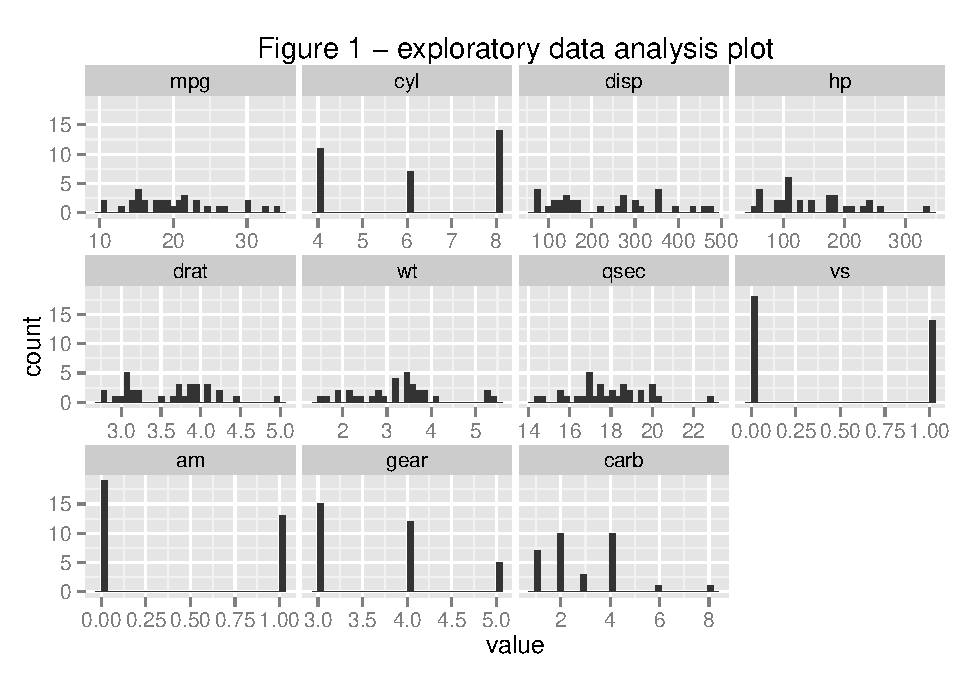
\includegraphics{project_files/figure-latex/unnamed-chunk-2-1} \end{flushleft}

\begin{flushleft}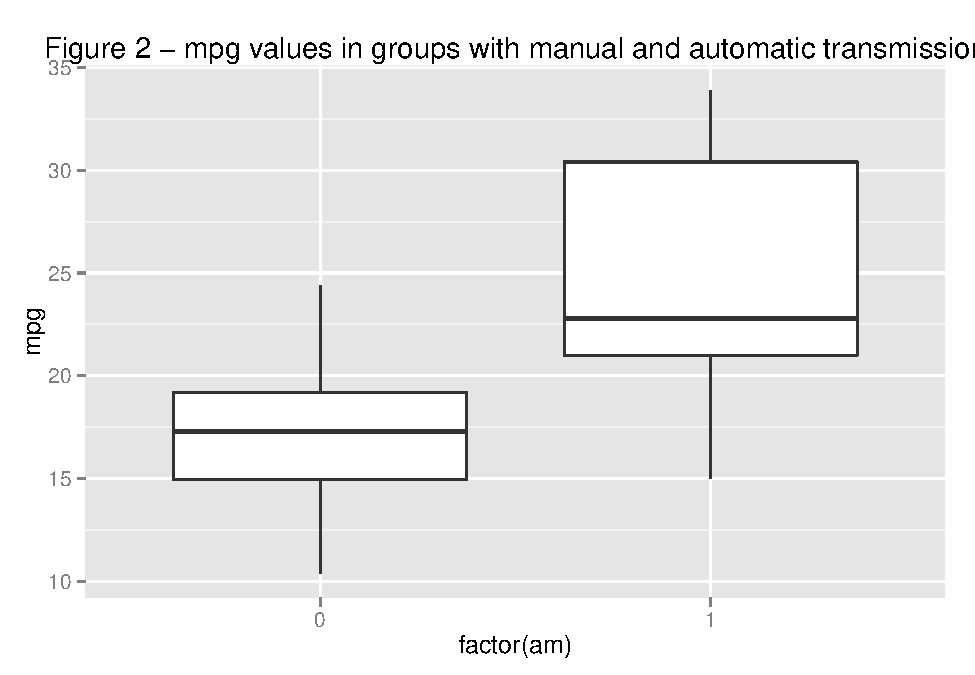
\includegraphics{project_files/figure-latex/mpg_automatic_vs_manual-1} \end{flushleft}

\begin{flushleft}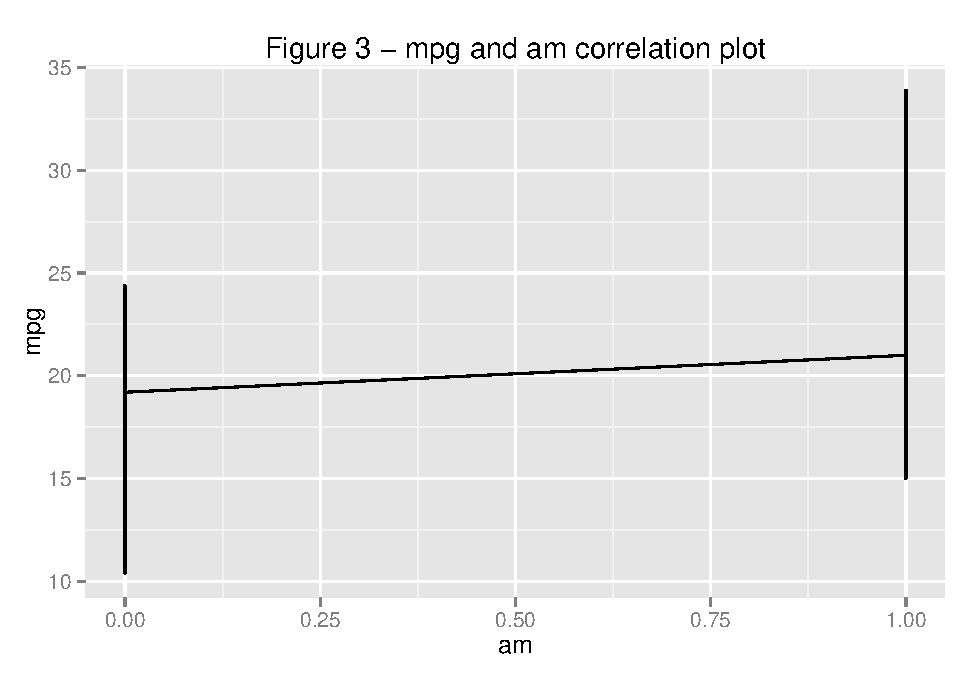
\includegraphics{project_files/figure-latex/mpg_am_correlation_plot-1} \end{flushleft}

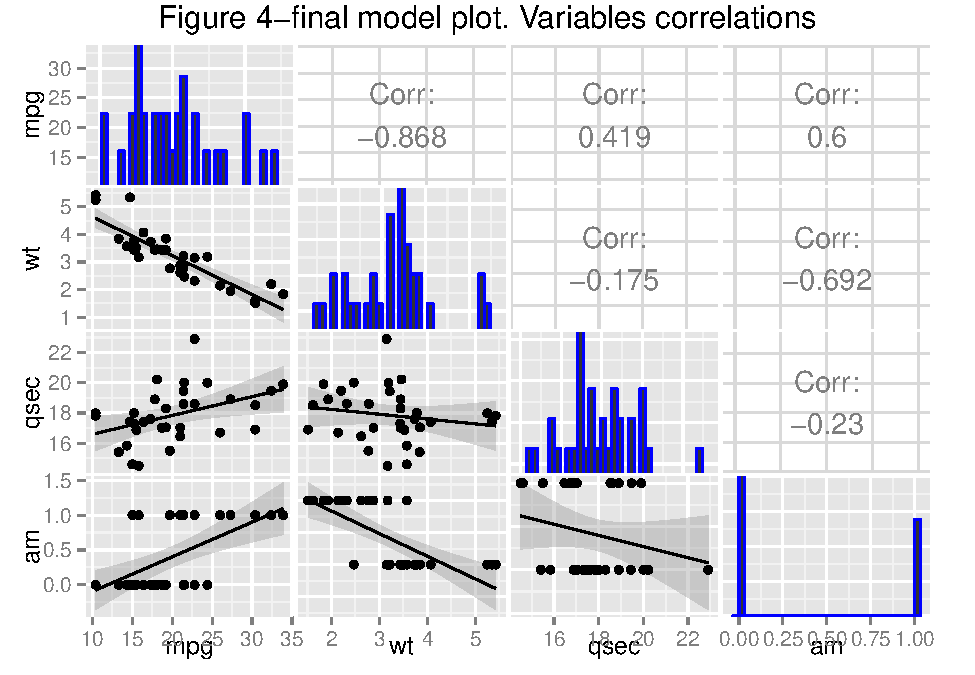
\includegraphics{project_files/figure-latex/final_model_plot_correlation-1.pdf}

\begin{flushleft}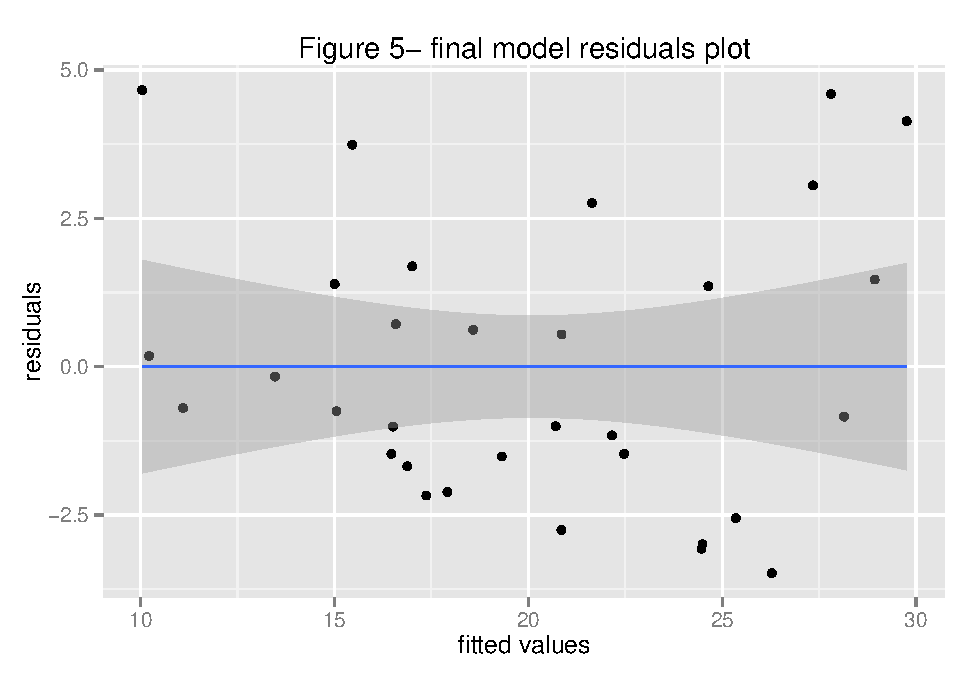
\includegraphics{project_files/figure-latex/final_model_plot_fit_results-1} \end{flushleft}

\end{document}
